%lit. survey I
\label{ch:calcPES}
The large variety of systems and effects studied with photoelectron spectroscopy led to the existence of diverse methods for theoretical modelling of the spectra \cite{PESbook, x-ray}.
In this work, the focus is put on steady-state photoelectron spectra of molecular systems with a size up to some tens of atoms.
As light source, here a classical ultra-violet or soft X-ray source with a discrete spectrum such as a gas discharge lamp or a laser is assumed where the strength of the applied electromagnetic field is weak and the kinetic energy of the outgoing electrons reaches at most tens of electronvolt but may become arbitrarily small.
\begin{table}[h]
\begin{center}
\begin{tabular}{|c|c|c|}
\hline
                  & Time-domain   & Frequency-domain \\
\hline
Field Str.& \begin{tabular}{c} weak to \\ strong \end{tabular} & weak \\
Method & \begin{tabular}{c} TDDO \cite{TD-do}\\ solving SE \\ Green's function \end{tabular} & 
        \begin{tabular}{c} R-Matrix \cite{Li-R,Li-R1,Burke,r-mat,R-mol1}\\ DO \cite{planeWave,DO_TDDFT} \\Green's Function \cite{GreenBayse,2phcederbaum} \\ Koopmans'\cite{dos,dos2,koopmansDFT} \end{tabular} \\
System Size & \begin{tabular}{c}atoms \cite{bauch1}, \\ diatomics \cite{bauch2,H2pDeCleva,saPonzi}\\ triatomics \cite{radau} \end{tabular} &
        \begin{tabular}{c}up to \\biomolecules \cite{bioPES}, \\ solid state \cite{Solid2,Leckey1992} \end{tabular} \\
Typical Problems  & \begin{tabular}{c}HHG \cite{hhg,zhangHHG,dromey_HHG}, \\Multiph. ionisation \\ attosec. dynam.\cite{as1,as2,as3,as4,as5,as6} \end{tabular} &
        \begin{tabular}{c} steady-state, \\ angle-res. PES \\time-res. PES \end{tabular} \\ 
QC$^{(a)}$ & \begin{tabular}{c}(TD)DFT, \\GASCI \cite{bauch1}, \\ EOM-CC \cite{CAPccEOM},\\ CASSCF \end{tabular}  &
        \begin{tabular}{c} CI\cite{ci1} \\ RASSCF \cite{MAgg,GrellKuehn,asscf1,asscf2}, \\ TD-DFT \end{tabular} \\
\hline
\end{tabular}
\end{center}
\caption{Overview of time- and frequency-domain methods and theyr typical applications.\\
  \small{$^{(a)}$QC: quantum chemical; GASCI: generalised active space configuration interaction; CASSCF: complete active space self-consistent field; EOM-CC: equation of motion- coupled cluster; RASSCF: restricted active space self-consistent field}.}
\label{tab:PEScat}
\end{table} 

A summary of methods that can be used to describe the most important scenarios arising in photoelectron spectroscopy is given in the Table \ref{tab:PEScat} and some of them are described in more detail in the following sections.
The main classification of these methods can be done dividing them into time and frequency domain.
These domains are related to each other via the Fourier transform but provide different pictures and properties.
Using a frequency-domain method, the Hamiltonian has to be diagonalised to obtain the states' energies and wave functions.
In contrast to this, in time domain the Hamiltonian is applied to an initial state to propagate the system in time.
Usually such a simulation needs several thousands of propagation steps to obtain reasonable accuracy.
Moreover, the joint treatment of bound and continuum states demands a large and flexible basis which makes time domain methods usually computationally very demanding and restricts their applicability to small systems as shown in the Table \ref{tab:PEScat}.
On the other hand, in frequency-domain the nonlinear response properties are neglected so that strong-field effects such as multiphoton ionisation and high harmonic generation (HHG) can not be treated.
Due to the different treatment of the system in both domains, they each have a set of methods that can be used and which are more or less specific to the domain as shown in the third column of Table \ref{tab:PEScat}.
The same holds for the quantum chemical methods available to treat the system.
\begin{wrapfigure}{R}{0.7\textwidth}
   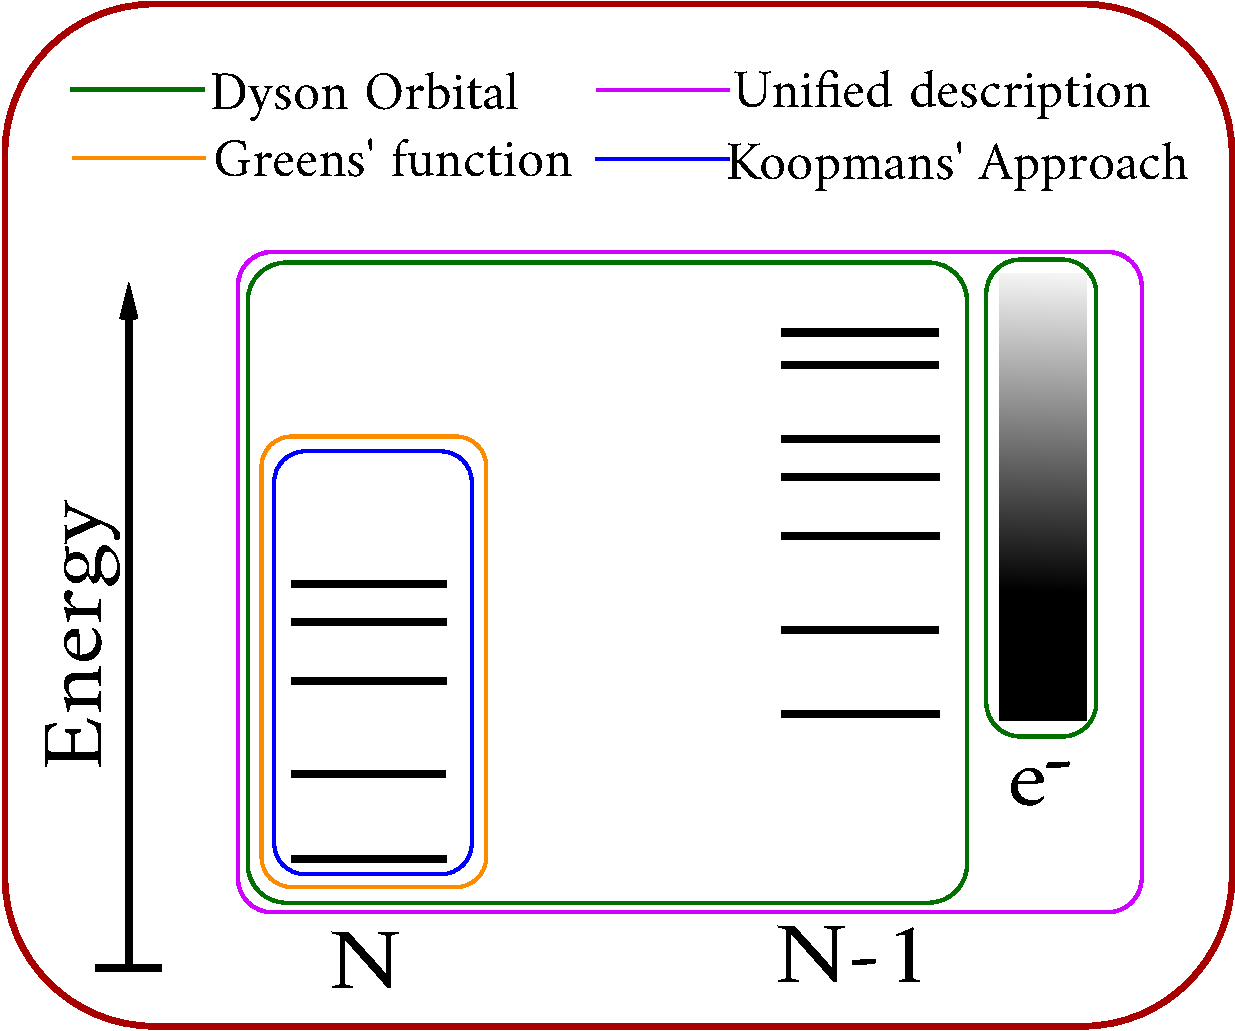
\includegraphics[width=0.7\textwidth]{Figures/Methods}
   \caption{Scheme of the system-representation used in the different methods.}
   \label{fig:PEScat}
\end{wrapfigure}
%\begin{table}
%\begin{tiny}\begin{tabular}{|c|c|c|c|c|c|}
%\hline
%                 & Field Str. & Method & System Size & Typical Problems &  QC$^{(a)}$ \\
%\hline
%\begin{tabular}{c}Time-\\ domain  \end{tabular}   &
%        \begin{tabular}{c} weak to \\ strong \end{tabular} & 
%        \begin{tabular}{c} TDDO \cite{TD-do}\\ SE \\ Green's function \end{tabular} &
%        \begin{tabular}{c}atoms \cite{bauch1}, \\ diatomics \cite{bauch2,H2pDeCleva,saPonzi}\\ triatomics \cite{radau} \end{tabular} & 
%        \begin{tabular}{c}HHG \cite{hhg,zhangHHG,dromey_HHG}, \\Multiph. ionisation \\ attosec. dynam.\cite{as1,as2,as3,as4,as5,as6} \end{tabular} &
%        \begin{tabular}{c}(TD)DFT, \\GASCI \cite{bauch1}, \\ EOM-CC \cite{CAPccEOM},\\ CASSCF \end{tabular} \\
%\hline
%\begin{tabular}{c}Frequency-\\ domain \end{tabular} & 
%        weak & 
%        \begin{tabular}{c} R-Matrix \cite{Li-R,Li-R1,Burke,r-mat,R-mol1}\\ DO \cite{planeWave,DO_TDDFT} \\Green's Function \cite{GreenBayse,2phcederbaum} \\ Koopmans'\cite{dos,dos2,koopmansDFT} \end{tabular} &
%        \begin{tabular}{c}up to \\biomolecules \cite{bioPES}, \\ solid state \cite{Solid2,Leckey1992} \end{tabular}& 
%        \begin{tabular}{c} steady-state, \\ angle-res. PES \\time-res. PES \end{tabular}& 
%        \begin{tabular}{c} CI\cite{ci1} \\ RASSCF \cite{MAgg,GrellKuehn,asscf1,asscf2}, \\ TD-DFT \end{tabular} \\
%\hline
%\end{tabular} \end{tiny}
%These nonlinear effects however usually do not play any role for classical light sources such as gas discharge or heat lamps and even most non-pulsed lasers.

Besides the distinction according to the domain, the methods can be also categorised according to the partitioning of the system they use which is sketched in Figure \ref{fig:PEScat}.
The simplest and crudest method is an approach derived from Koopman's theorem where only the ground state of the un\-ion\-ised state is considered which is visualised in Figure \ref{fig:PEScat} by the fact that the box for this method is only at the $N$-electron system.
Similarly, also the Green's function approach treats only the initial state but accounts for electron relaxation and thus correlation effects during ionisation due to its quasi-particle picture.
In the DO formalism, in contrast, the final state is treated explicitly, using a partitioning into the bound $N-1$-electron state $|\Psi^{N-1}\rangle$ and the FEF $|\Psi^\text{el}\rangle$.
%The wave function of the initial state $|\Psi^{N}\rangle$ moreover is obtained in a separate calculation; so in total three different calculations are used which is represented by the three boxes in Figure \ref{fig:PEScat}.
Finally a large class of methods treat the system uniformly, using a joint treatment for the bound and continuum states as indicated by the single box in Figure \ref{fig:PEScat}.
%Typically time-domain methods are in this last group of methods.

The Koopmans' approach is, at least among the frequency domain methods, the most prominent representative \cite{Koerzd1,PottsHolland,dos,dos2}.
In this scheme, the systems ground state is computed with a self-consistent field quantum mechanical method to obtain the one-electron binding energies.
The photoelectron spectrum is than estimated using the orbital energies as the transition energies and using uniform intensities.
Although this method has shown to be in qualitative agreement with experiments for different systems \cite{Koerzd1,Koerzd2, EggerKronik,PottsHolland,YepesJaque}, it breaks down in case of strong electron correlation \cite{2phcederbaum,2phcederbaum2} due to relaxation of the orbitals upon ionisation.
%Since the estimation of the role of correlation effects can only hardly be estimated in advance, this method has only poor predictive character.
This method is characterised by its low computational costs and robustness and, thus, is well-suited for very large systems such as solid state problems where calculations beyond ground-state DFT are very demanding or not feasible at all.

In the following sections, the most important methods will be briefly introduced according to their affiliation to the groups distiguished in Figure \ref{fig:PEScat}.
First, in section \ref{ch:gf} the working equations of the Green's function approach are introduced to give a fundamental understanding of this group of methods.
Thereafter, in section \ref{ch:r-mat} several approaches both in time- and frequency-domain are described that use a unified descrption of the complete $N$-electron system.
Finally the DO formalism is derived in more detail, since it is the method of choise in this work, in section \ref{ch:do}.

\section{Green's Function Approach}
\label{ch:gf}
From a formal point of view, the computation of photoelectron spectra using the Green's function approach is similar to the use of Koopmans' approach since in both methods only the ground state of the unionised system is considered.
However, the level of theory achievable when using Green's functions is much higher.

In contrast to most other quantum-chemical methods, in the Greens' function approach expectation values for a given operator $\hat{O}$ are not computed as a scalar product $\langle \Psi^N |\hat{O} | \Psi^N \rangle $ with the wave function $|\Psi^N\rangle$ of the $N$ electron state of interest, but by contour integrals with the Greens' function \cite{bookGF, 1pGFcederbaum}.
Thereby the (one particle) Greens' function is a matrix $\mat{G}$ whose elements are defined as
\begin{equation} \label{eq:defGF}
G_{i,j}(t,t')= -\text{i}\langle \Psi^N | \hat{T}\left(\hat{a}_i(t)\hat{a}_j^\dagger(t')\right)|\Psi^N\rangle 
\end{equation}
with the creation operator $\hat{a}^\dagger_j (t)=e^{\text{i}\hat{H}t}\hat{a}^\dagger_j e^{-\text{i}\hat{H}t}$ of an electron in state $j$ at time $t$ in Heisenberg picture and the annihilation operator $\hat{a}(t)=e^{-\text{i}\hat{H}t}\hat{a}_j e^{\text{i}\hat{H}t}$ respectively.
$\hat{T}$ is the Dyson time ordering operator that orders the operators $\hat{a}$ and $\hat{a}^\dagger$ by their time arguments to ensure that the operator with smaller time argument acts first \cite{bookGF}.
Hence, the Greens' function can be interpreted as an additional electron (or hole, depending on the time ordering) propagating from $t'$ to $t$ in a system described by the Hamiltonian $\hat{H}$ \cite{bookGF}.

%In this approach the calculation of photoelectron spectra is formulated such that the poles and residues of the Fourier transformed Greens' function are searched.
%This becomes clear when writing the time-ordering operator in equation (\ref{eq:defGF}) explicitly
To find an expression of the Green's function (\ref{eq:defGF}) from which the transition energies and intensities can be extracted, it needs to be reformulated.
In the first step, the time ordering operator is written explicitly which results in 
\begin{equation} \label{eq:GF}
G_{i,j}(t,t')= \text{i}\langle \Psi^N | \hat{a}_j(t)\hat{a}^\dagger_i(t') |\Psi^N\rangle \Theta(t-t') -
                   \text{i} \langle \Psi^N | \hat{a}^\dagger_i(t')\hat{a}_j(t) |\Psi^N\rangle \Theta(t'-t).
\end{equation}
Inserting the closure relation $\hat{1}=\sum_k |\Psi^M_k\rangle\langle \Psi^M_k |$, where $M=N\pm 1$ and $|\Psi^M_k\rangle$ describes a bound state, between the operators in both terms of (\ref{eq:GF}), the Lehmann representation \cite{bookGF} is obtained whose Fourier transform is
\begin{equation}\label{eq:gfSpect}
G_{i,j}(\omega)=\text{i} \sum_k\frac{\left|\langle \Psi^N | \hat{a}_j|\Psi^{N+1}_k \rangle \right|^3}{\omega-(E_k^{N+1}-E^N)+\text{i}\nu}-
                \text{i}\sum_k\frac{\left|\langle \Psi^N | \hat{a}^\dagger_i|\Psi^{N-1}_k \rangle \right|^2}{\omega+(E_k^{N-1}-E^N)-\text{i}\nu},
\end{equation}
where $\nu$ is a small parameter arising from calculation of principal value and $\omega$ denotes the argument of the Fourier transform while $E^N$ and $E_k^M$ are the energies of the $N$-electron ground stated $|\Psi^N\rangle$ and of the $k$-th $M$-electron state $|\Psi_k^M\rangle$, respectively.
In this form, the second sum corresponds to transitions in the PES: the nodes of the denominator (poles of the Greens' function) can be easily assigned to the ionisation potentials and, thus, the transition energies in photoelectron spectra.
Further, the integrals in the nominator are equivalent to the sudden approximation derived in chapter \ref{ch:sa} and hence provide a good approximation to the transition strengths.
The terms in the first sum correspond to the respective quantities of electron detachment \cite{1pGFcederbaum}.

However, computing the Greens' function is a demanding task which is of similar complexity as the computation of a solution to the SE.
Over the years several approaches were developed of which the algebraic diagrammatic construction \cite{1pGFcederbaum} and the equation of motion \cite{PottsHolland,1pGFcederbaum} are the most prominent.
In the diagrammatic construction one starts with an initial zeroth order Greens' function $\mat{G}^0(\omega)$ constructed in a Hartree-Fock basis and corrects it iteratively by the term $\mat{G}^0(\omega)\mat{\Sigma}(\omega)\mat{G}(\omega)$, where $\mat{\Sigma}(\omega)$ is the self-energy, an effective potential that is used to recover electron correlation and relaxation effects \cite{GreenBayse}.
The self-energy usually is expanded in a perturbation series with respect to Feynman diagrams with increasing number of vertices and is exact in the limit of infinite terms \cite{bookGF,cederbADC}.
The one-particle energies, Coulomb matrix elements and overlap integrals are obtained from self-consistent field (SCF) calculations \cite{1pGFcederbaum} \textit{e.g.} on the HF-level \cite{GreenBayse} but (TD)DFT or any other quantum chemical method can be used as well via the GW-approach \cite{gf_intro,hedinGW}.
Being much easier to compute, the Hartree-Fock basis has the disadvantage that only single configurational electronic states can be treated.

On the other hand, an important advantage of the Greens' function method is that the transition energies are computed directly whereas in most other methods they are calculated as the difference of the initial and final state energies.
The latter approach however can lead to errors in the electronvolt range when the difference in the correlation energy is badly estimated \cite{1pGFcederbaum}.

%Another, yet similarly simple approach used in cases where only few electronic transitions are present is to fit the intensity to experimental data \cite{winterWater,hemberg1}.
%This is especially used when the vibrational structure is resolved.
%
%Here, two different approaches are possible.
%While most methods use Fermis Golden Rule 
%\[  \sigma(\omega)\propto |\langle |\hat{mu}|\rangle|^2 g(E_f-E_i+h\nu -\omega)
%\]
%where the intensity of the transitions is calculated via the dipole matrix elements, the other route is
%via the complex polarisability $\alpha(\omega)=\int_{IP}^\infty \frac{df(\epsilon)}{\epsilon^2-\omega^2}$. 
%In the latter case, the spectrum is obtained via
%\[ \sigma(\omega)=\frac{4\pi \omega}{c} Im(\alpha(\omega)).\]
% Some of them are especially generated for special geometries such as the R-matrix method described in chapter \ref{ch:r-mat}, others such as the Greens' function or Dyson orbital formalism introduced in the chapters \ref{ch:gf} and \ref{ch:do} respectively are more general but can not reach the same accuracy.
% Besides different classes of molecules, also the light irradiation considered can differ: Some methods are especially designed for large intensities \textcolor{green}{sources} or kinetic energies in the relativistic regime \textcolor{green}{source}.
 %In this work, however, only methods applicable in more moderate regimes are considered, meaning that perturbation theory is applicable and the kinetic energy of the photoelectron is considered to not above the $keV$-range.
%\section{Methods where electron is treated in same footing as bound states}
%\section{Methods with Unified Description of Bound and Free States}
\section{Combined Bound and Continuum State Representation}
\label{ch:r-mat}
%Another large class of methods for computing photoelectron spectra uses perturbation theory in frequency domain or the dipole autocorrelation function in time domain respectively.
%In frequency domain thereby the initial state and final state are described therein each as $N$ electron systems with a uniform scheme, requiring the basis set to be formulated general enough to represent bound as well as free states.
In contrast to the Greens' function method, in which the explicit description of the FEF  omitted, a large group of methods describes the full $N$-electron system before and after the ionisation, respectively (see Figure \ref{fig:PEScat}).
In this section a selection of such methods is presented.
The treatment of bound and continuum states, however, requires a very flexible formalism whose large computational costs restrict its applicability to small systems that often fulfil certain symmetry-requirements and have a small amount of electrons.

The most prominent representative of this class in frequency domain is the R-matrix method \cite{r-mat, r-mat2,Burke}.
Its general idea is to conduct a partition of space into regions which are treated differently and connected by explicit boundary conditions to ensure smoothness of the wave function.
These regions are constructed with concentric spheres, restricting the symmetry of wave functions in this scheme.
Nonetheless it is found to be applied not only to atoms \cite{Li-R,Li-R1,Li-R2} but also to small molecules \cite{R-mol1,R-mol2}.
In the R-matrix formalism the inner region is chosen large enough to contain the bound part of the $N$-electron function that is usually represented by a configuration interaction (CI) expansion of Slater determinants (SDs), using a linear combination of atomic orbitals (LCAO) basis or a grid representation \cite{Burke}.
The FEF is commonly described by a linear combination of bound orbital type functions and continuum functions such as Coulomb waves \cite{r-mat, r-mat2}. %or a product description of spherical Harmonic and a spline-based radial function.
%a antisymmetrised product of Coulomb type wave function with ...\cite{r-mat,r-mat2}.
\begin{wrapfigure}{r}{0.48\textwidth}
   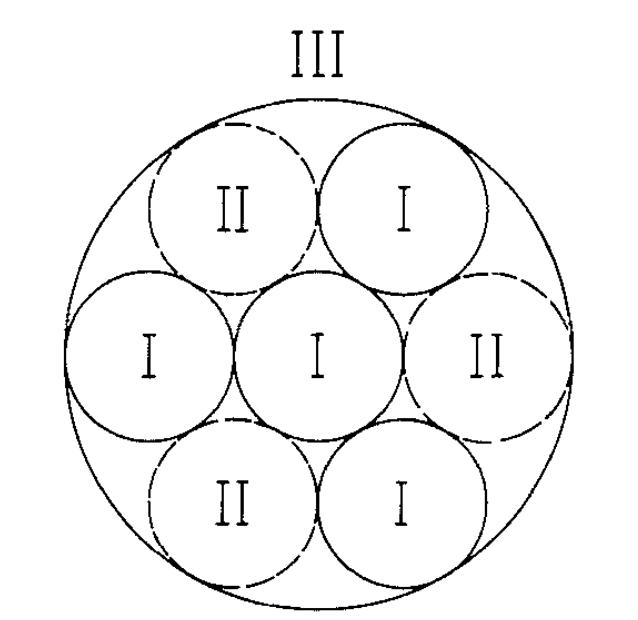
\includegraphics[width=0.48\textwidth]{Figures/JohnsonSpheres}
   \caption{Schematic view of the space partition scheme used by Johnson for a four-atomic molecule:
    I: atomic, II: interatomic and III: outer region \cite{johnson}.}
   \label{fig:johnson}
\end{wrapfigure}
In the outer region, an expansion in Coulomb waves is used to ensure the asymptotically correct behaviour.
In addition to the inner region and the asymptotic outer region further intermediate regions can be added  where the FEF is represented by a multipole-radiation expansion which is a polynomial of inverse powers of the distance to the centre \cite{Burke}.

%in which the multipole functions can be added\cite{Burke}.
A generalisation to non-spherical systems is employed, \textit{e.g.}, by Johnson \cite{johnson} who used different kinds of non-concentric spheres.
One set spheres is centred at atoms while others are placed in the interatomic regions such that the space is filled as dense as possible as shown in Figure \ref{fig:johnson} for a molecule with four atoms.
Each atom is located in the centre of a circle denoted as I while the circles II fill the interatomic space.
An outer sphere surrounds the molecule to account for the asymptotic region similar to the asymptotic region in R-matrix theory.
In this scheme, the exchange-correlation is treated on an approximate level \cite{slaterJohn} and is spherically averaged, resulting in a description that is equivalent to the muffin-tin potential which is a well-known model in solid state physics \cite{MufTin,MufTin1}.
The continuity of the wave-functions as well as their derivatives is ensured over the regions via multiple-scattered-wave theory \cite{johnson}.
%Thereby the potential energy contains besides the Coulomb term also a statistical approximation of the exchange correlation of the form
%\begin{equation}
 %V_{x\alpha}(\vec{r}) = -6\alpha\left( \frac 38 \pi \rho(\vec{r})\right)^{\frac 13} 
%\end{equation}
%where $\rho(\vec{r})$ is the electron density and $\alpha$ is a parameter that is chosen differently for each element.
%In each of the regions the potential %energy is expanded in a superposition of spherical harmonics that is truncated after the $l=0$ term which is equivalent to the muffin-tin potential which is well-known especially for solids \cite{MufTin,MufTin1}.
The wave-functions are chosen in each region as a one-centre expansion in spherical coordinates of the form
\begin{equation} \label{eq:radSE}
\Psi(r, \theta, \phi) =\sum_{l=0}^{l_\text{max}}\sum_{m=-l}^l c_{l,m} R_l(r) Y_l^m(\theta, \phi)
\end{equation}
where $r,\theta,\phi$ are the spherical coordinates and $Y_l^m(\theta,\phi)$ are the spherical Harmonics \cite{Lifschitz} and the radial function $R_l(r)$ is a solution of the radial SE 
\begin{equation} \label{eq:radSEeq}
\frac{\partial^2 R(r)}{\partial r^2} + \left( 2\left(E-V(r)\right) + \frac{l(l+1)}{r^2} \right)R(r)=0
\end{equation}
with the respective spherically averaged potential $V(r)$ \cite{johnson}.

%A similar approach is to describe the bound and free states at the same level as applied by DeCleva \textit{et al.}  $H_2^+$\cite{H2pDeCleva}.
An approach applied by DeCleva \textit{et al.} to $H_2^+$ \cite{H2pDeCleva} and benzene \cite{DeClevaBenzene} refrains from the use of spheres, allowing for more general boundaries between the inner and outer regions.
Here the FEFs are globally represented as the one-centre expansion (\ref{eq:radSE}) where $R(r)$ is expressed by a B-spline basis. % (details about the spline description are given in section \ref{ch:dvr}).
An advantage of the spline-based description is that smoothness at the interface between the regions is ensured intrinsically.

Another scheme in frequency domain is used by Richards and Larkins \cite{richardsFD} with a hybrid ansatz: The bound states of the H$_2$ molecule are described in the common LCAO scheme and the FEF is described by the product ansatz $\Psi(\vec{r}) = R(r,\theta) e^{im\phi}$, which is a generalisation of (\ref{eq:radSE}), where $R(r,\theta)$ is obtained from a two-dimensional SE on a regular grid using a finite difference (FD) scheme.
In contrast to the previously described methods, here no partition of space is performed but instead a finite box with Dirichlet boundary conditions is used.
Moreover, the FEF is treated on the HF-level, neglecting correlation effects \cite{richardsFD}.

Similar descriptions are used in time domain by several authors \cite{CAPccEOM, bauch1, taoDVR}.
Even though they are much more demanding than calculations in frequency domain, time domain methods can predict strong-field effects and are used to simulate attosecond dynamic which is both not achievable using frequency-domain methods.

An important difference between time- and frequency-domain methods of practical use is that in time-domain unbound particles are described by a wave packet and hence as a localised function.
Moreover, at short times after ionisation the continuum states often can be assumed to be of similar spacial extend as bound states, allowing the basis to be a linear combination of bound state functions but having a complex energy whose real part introduces oscillations and the imaginary part damps the wave function, leading to a finite lifetime of the function \cite{CAPccEOM}.
Moreover a complex absorbing potential (CAP) (discussed in chapter \ref{ch:cap} in more detail) is most often applied, ensuring that the continuum states can be described by bound-state functions by cutting off that part of the wave function which is not localised at the molecule anymore.
Due to these considerations the LCAO basis can be used for the description of the free particles as well, see \textit{e.g.} Jagau \textit{et al.} \cite{CAPccEOM}.
In other simulations, grid-based descriptions are chosen using symmetry-adapted coordinate systems \cite{radau,jacobi, hyperspheric,taoDVR}, allowing for a product ansatz similar to (\ref{eq:radSE}) and hence a reduction in dimensionality.
%In other simulations, a grid-based description is chosen using spherical, elliptical or hyperspherical coordinates, allowing ng for a product ansatz and hence a reduction to one dimension.
On the remaining one-dimensional grids often a discrete variable representation (DVR) (described in section \ref{ch:dvr} of this thesis) is chosen.
As an example, Yip \textit{et al.} \cite{yipDVR} simulate double ionisation of atomic beryllium in spherical coordinates, using the expansion (\ref{eq:radSE}) where $R(r)$ is separated into two regions in which a DVR and a finite element DVR (FE-DVR) scheme are used respectively.
As other examples, Tao \textit{et al.} \cite{taoDVR} as well as Bauch \textit{et al.} \cite{bauch1, bauch2} use the FE-DVR basis in spheroidal coordinates.

The examples introduced above represent only a small fraction of the methods used to describe photoionisation in frequency and time domain.
But a drawback that is common to these methods is that a large number of continuum functions is required which are correlated with the bound electrons and thus lead to a computationally expensive description of the system.
To overcome this drawback, in the DO formalism that is presented in the coming section the description of bound and continuum states is separated into separate problems.

%\textcolor{red}{This is by far not a complete list; are these at least the most important methods?}
%
%A different technique is used by Son \textit{et al.} who use time dependent density functional theory (TDDFT) based on a finite volume scheme instead of the usual LCAO approach.
%Thereby no asymptotic region is utilised, instead the region of interest is chosen by setting a sphere with a given radius around each atom \cite{Son_Chu0,Son_Chu}.

%Sato \textit{et al.}\textcolor{green}{sources} 
\section{The Dyson Orbital Formalism}
\label{ch:do}
The Dyson orbital (DO) formalism can be considered as an approximation to the methods described above.
Here the free and bound states are described separately, see Figure \ref{fig:PEScat}, using a product ansatz.
Using such a separation leads to a neglect of correlation effects between the outgoing electron and the bound states and is often denoted as sudden ionisation limit \cite{ezDyson,MAgg}.
Moreover, non-linear effects as well as recombination transitions are not considered within DO theory.
An important advantage, however, is that the overlap between the initial state and the bound part of the final state is formulated as a one-electron quantity, called DO which can be used to simplify the description of the photoionisation process.
%reducing the computation of the dipole matrix elements to a one-electron integration.
Usually the DO scheme is considered in the frequency domain, but a time domain formulation exists as well and is described in the following section \cite{TD-do}.
%The DO therein can be interpreted as a quasi-particle that is removed from the molecules; incorporating multi-particle effects such as electron relaxation or instantaneous excitation of other electrons.

\subsection{Time-dependent Dyson Orbitals}
%There are several approaches towards Dyson orbitals.
%Here we will mainly follow the derivation of Gritsenko \textit{et al.} \cite{TD-do}, starting from an exact time-dependent expression.
%Here we will mainly follow the derivation of Gritsenko \textit{et al.} \cite{TD-do}, starting from an exact time-dependent expression.
%Thereby the $j$-th time dependent Dyson orbital (TDDO) is defined as the overlap integral of the $j$-th final ionised state $\Psi_j^{N-1}^\dagger(\vec{r}_2,\hdots,\vec{r}_N)$ with the unionised initial $N$-electron state $\Psi^{N}(\vec{r}, \vec{r}_2,\hdots,\vec{r}_N)$
%\begin{equation}
%\Psi_\text{DO}^j(\vec{r}) = \sqrt{N} \int \Psi_j^{N-1}^\dagger(\vec{r}_2,\hdots,\vec{r}_N)
%                                           \Psi^{N}(\vec{r}, \vec{r}_2,\hdots,\vec{r}_N)
%                            d\vec{r}_2 \hdots d\vec{r}_N .
%\end{equation} 
A good starting point for the DO formalism is an expansion of the time-dependent $N$-electron function $|\Psi^N(t)\rangle$ (omitting the spacial coordinates for brevity) in the form
\begin{equation} \label{eq:DOexpansion}
%\Psi^N(\vec{r}, \vec{r}_2, \hdots,\vec{r}_N, t)=\frac{1}{\sqrt{N}} \sum_k \Psi^k_\text{DO}(\vec{r},t) \Psi_k^{N-1}(\vec{r}_2, \hdots,\vec{r}_N)e^{\text{i}E_k^{N-1}t}
| \Psi^N (t)\rangle =\frac{1}{\sqrt{N}} \sum_k |\Psi_k^{DO}(t)\rangle | \Psi^{N-1}_k \rangle e^{iE_k^{N-1}t}
\end{equation}
where $E_k^{N-1}$ are the energies of the $N-1$-electron bound states described by the time-independent wave functions $|\Psi_k^{N-1}\rangle$ that are complete in the space of $N-1$-electron wave-functions.
The expansion coefficients $|\Psi_k^{DO}(t)\rangle$ have the dimensionality of a one-particle function and are denoted as time-dependent DO (TDDO).
An important feature of the expansion (\ref{eq:DOexpansion}) is that the dynamics of the $N$-electron system is reduced to a system of one-electron quantities $|\Psi_k^\text{DO}(t)\rangle$, propagated according to the electronic SE \cite{TD-do}.
%\begin{equation}
%\text{i}\frac{\partial}{\partial t}|\Psi_j(t)\rangle =
%\left{-\frac 12 \nabla^2 + \hat{v}_\text{ext}(\ver{r},t) +\Delta_j(t) \right} |Psi_j(t)\rangle
%\end{equation}
In this approach the interaction of the DO with the bound states is approximated by the mean-field electrostatic potential (ESP) \cite{TD-do}, neglecting exchange and correlation.

The physical interpretation of the TDDO becomes clear when regarding its definition, given by the $N-1$-electron integral
\begin{equation} \label{eq:TDDO}
%\Psi^k_\text{DO}(\vec{r},t) = \sqrt{N} \int \Psi_k^{N-1 \dagger}(\vec{r}_2,\hdots,\vec{r}_N) e^{\text{i}E_k^{N-1}t}
                              %\Psi^N(\vec{r}, \vec{r}_2, \hdots,\vec{r}_N, t) d\vec{r}_2,\hdots d\vec{r}_N.
|\Psi_k^\text{DO}(t)\rangle =  e^{\text{i}E_k^{N-1}t}\sqrt{N} \langle \Psi_k^{N-1} |\Psi^N(t) \rangle_{N-1}.
\end{equation}
The remaining coordinate (\ref{eq:TDDO}) belongs to the photoelectron since $|\Psi^{N-1}(t)\rangle$ is restricted to the description of bound states.
Considering eq. \ref{eq:TDDO} in a frozen orbital approximation, \textit{i.e.} one-electron ionisation, the TDDO corresponds to the photoelectron.
However, relaxation effects lead to non-orthogonal orbitals of the $N$- and $N-1$-electron systems and thus lead to additional contributions to the TDDO.
Therefore, when considering relaxation effects, the TDDO is a quasi-particle describing the electron that is ionised, including relaxation and correlation effects \cite{ezDyson,TD-do}.
%Thereby especially three time slices are interesting: $t<0$ \textit{i.e.} before the ionisation , $t=0$ and the limit of $t\rightarrow \infty$.
%For $t<0$ hence the expression (\ref{eq:DOexpansion}) describes the unionised system in its initial state where the DO is a molecular orbital and equation (\ref{eq:DOexpansion}) is a way to write a Slater determinant (SD).
%In the limes of $t\longrightarrow \infty$ thereby $|\Psi_k^{N-1}\rangle$ describes the ionic remainder in a state $k$ and hence the TDDO is the free electron function (FEF) whose energy is determined by the laser pulse which ionised the system as well as the energy $E_k^{N-1}$.
%However, due to relaxation and correlation effects, the orbitals in the final states are different from those in the $N$ electron state and hence these changes are also contained in the TDDO.
%For the case $t=0$ these relaxation effects also are included in the TDDO but the FEF did not change its wave function with respect to the ionised orbital hence its wave function is that of the removed electron, amended by combination and relaxation effects. \\ \\
%Thereby, this formalism resolves two main problems of time propagation using standard TDDFT which are the missing memory effects due to an approximate exchange potential that depends on the current density only. % this is resolved because in the 1-particle EOMs only static electron-electron interaction potentials occur.
%The second problem often occurring is that usual TDDFT is not able to predict correlated multiple ionisations which can be resolved with this formalism as well \cite{TD-do}.

\subsection{Time-independent Dyson Orbitals}
Working in frequency domain, no propagation needs to be considered.
Instead, the quantity of interest here is the stationary DO which corresponds to the TDDO at $t=0$.
From eq. \ref{eq:TDDO} the DO can be interpreted as quasi-particle that is ejected by the irradiating light \cite{ezDyson}.

While for the TDDO only the general expressions were shown, in this section, since the time-independent DO formalism is used within this work, a more detailed derivation of the expressions is done.

%To see the benefit of using the DO formalism for computing photoelectron spectra, we start with the photoelectron cross section in atomic units
The main advantage of this formalism in frequency-domain becomes clear when the photoelectron cross-section is considered.
In the Fermis' Golden Rule \cite{fgr} formulation, which assumes the wavelength to be much larger than the characteristic size of the system under study and weak irradiating light-field, the cross-section for the transition between an initial $i$ and final $k$ states is in atomic units \cite{richardsFD,MAgg}
\begin{equation} \label{eq:sigma}
\sigma(\epsilon) =\frac 23
           \sum_k (\varepsilon +E_k-E_i)\left| \langle \Psi^N_i | \vec{\hat{d}} | \Psi^N_{k}\rangle \rho(\varepsilon)
\right|^2  
             \propto \sum_k \left|  \vec{D}_k \right| ^2
\end{equation}
where $\epsilon=h\nu-(E_k-E_i)$ is the kinetic energy of the photoelectron that is determined by the photon energy $h\nu$ and the energies $E_\alpha$ of the initial unionised state $|\Psi^N_i \rangle$ and the final ionised state $|\Psi^N_k\rangle$ which includes all electrons, further $\vec{D}_k=\langle \Psi^N_i | \vec{\hat{d}} | \Psi^N_{k}\rangle$ is the transition dipole moment and $\rho(\varepsilon)$ is the density of final states which is in the following assumed to be a delta function.
Writing the initial and final states each as SDs
\begin{subequations} \label{eq:SDs} \begin{align}
   |\Psi^N_i\rangle &= \hat{A}_N | \Phi_{i,1} \hdots \Phi_{i,N} \rangle \\
   |\Psi^N_k \rangle &= \hat{A}_N | \Phi_{k,1}\hdots \Phi_{k,N-1} \Psi_k^\text{el} \rangle
\end{align}\end{subequations}
where $\hat{A}_N$ is an $N$-electron antisymmetrisation operator, $|\Phi_{k,j}\rangle$ are the $j$-th (Kohn-Sham) orbitals and $\Psi_k^\text{el}$ is the FEF.
The index $k$ enumerates the final states which can have an arbitrary electron configuration here.
The dipole operator $\hat{\vec{d}}$ is a one-electron operator that can be written as $\hat{\vec{d}}=\sum_{j=1}^N \hat{\vec{d}}_j$ where $\hat{\vec{d}}_j=\vec{r}_j$ in length gauge or $\hat{\vec{d}}_j=\nabla_j/(\varepsilon +E_k-E_i)$ in velocity gauge respectively \cite{richardsFD}.

Using the SD representations (\ref{eq:SDs}), the integral $\vec{D}_k$ in eq. (\ref{eq:sigma}) can be written as
\begin{equation} \label{eq:derDO1}
\vec{D}_k = \langle
\Phi_{i,1}  \hdots\Phi_{i,N} | \hat{A}_N \sum_{j=1}^N\hat{\vec{d}}_j \hat{A}_N |
\Phi_{k,1}\hdots\Phi_{k,N-1} \Psi_\text{el} 
\rangle ,
\end{equation}
where hermiticity of the antisymmetrisation operator is used.
The expression (\ref{eq:derDO1}) can be further expanded taking into account that $\hat{A}_N$ commutes with the dipole operator and making use of the relation $\hat{A}_N\hat{A}_N=\sqrt{N!}\hat{A}_N=\sum_P (-1)^p \hat{P}$ where the sum goes over all permutations $\hat{P}$ of electron indices with parity $p$
\begin{align} \label{eq:derDO2}
\vec{D}_k & = \sqrt{N!}\sum_P (-1)^p \sum_{j=1}^N \langle
\Phi_{i,P(1)}\hdots\Phi_{i,P(N)} |\hat{\vec{d}}_j |
\Phi_{k,1}\hdots\Phi_{k,N-1} \Psi_\text{el}  \rangle  \\
  & = \sqrt{N!}\sum_P (-1)^p \sum_{j=1}^N 
  \langle \Phi_{i,P(j)} | \hat{\vec{d}}_j | \Phi_{k,j} \rangle
          \langle \Phi_{i,P(1)}  |\Phi_{k,1}   \rangle
  \hdots  \langle \Phi_{i,P(j-1)}|\Phi_{k,j-1} \rangle \\
  & \times\langle \Phi_{i,P(j+1)}|\Phi_{k,j+1} \rangle
          \langle \Phi_{i,P(N-1)}|\Phi_{k,N-1} \rangle
  \hdots  \langle \Phi_{i,P(N)}  |\Psi_\text{el}\rangle 
\end{align}
where $P(j)$ is a permutation of the $j$-th orbital.
Thereby the term $j=N$ differs qualitatively from the others since the dipole operator acts on the FEF.
Hence the sum can be reordered to obtain
\begin{align} \label{eq:fullDO}
  \vec{D}_k & = 
  \underbrace{\sqrt{N!}\sum_P (-1)^p 
          \langle \Phi_{i,P(1)}  |\Phi_{k,1}    \rangle
  \hdots  \langle \Phi_{i,P(N-1)}|\Phi_{k,N-1}  \rangle
  \langle \Phi_{i,P(N)} }_{\langle \Psi_k^\text{DO}|} | \hat{\vec{d}}_j | \Psi_\text{el} \rangle + \nonumber \\
  & 
       \sqrt{N!}\sum_P (-1)^p \sum_{j=1}^{N-1} 
          \langle \Phi_{i,P(1)}  |\Phi_{k,1}    \rangle
  \hdots  \langle \Phi_{i,P(j-1)}|\Phi_{k,j-1}  \rangle
  \langle \Phi_{i,P(j)}|\hat{\vec{d}}_j |\Phi_{k,j}\rangle \times \nonumber \\
  &       \langle \Phi_{i,P(j+1)}|\Phi_{k,j+1}  \rangle
  \hdots  \langle \Phi_{i,P(N-1)}|\Phi_{k,N-1}  \rangle
  \langle \Phi_{i,P(N)}| \Psi_k^\text{el} \rangle
\end{align}
where the first sum is denoted as DO and the second as conjugate DO respectively \cite{saPonzi}.
To reduce the large amount of integrals therein, the strong orthogonality approximation is applied under the assumption that the overlap 
\begin{equation}
 \langle \Phi_{i,j}  |\Psi_\text{el}\rangle=0 \quad \forall\, j=1,\hdots, N
\end{equation}
of the FEF with all bound states vanishes.
This is strictly valid if $|\Phi_{i,j}\rangle$ and $|\Psi^\text{el}\rangle$ would correspond to the same Hamiltonian.
But in most cases the relaxation of the orbital $|\Phi_{i,j}\rangle$ is small, leading to a small but non-zero overlap with the FEF \cite{saPonzi,GrellKuehn}.
Applying the strong orthogonality condition leads to the drop out of the second sum in \eq{eq:fullDO} and the transition dipole moment simplifies to
\begin{align} \label{eq:sigma_do}
\vec{D}_k&= \sum_p (-1)^P \langle \Phi_{i,P(1)}  |\Phi_{k,1} \rangle
            \hdots  \langle \Phi_{i,P(N-1)}|\Phi_{k,N-1} \rangle
                   \langle \Phi_{i,P(N)} |\hat{\vec{d}}_j |\Psi_k^\text{el}\rangle \nonumber \\
    &= \langle \Psi_k^\text{DO}| \hat{\vec{d}}_j| \Psi_k^\text{el}\rangle
\end{align}
%\textcolor{blue}{?? At the moment, there is no equation of the DO to reference. Write it differently?}
which corresponds to the definition of the TDDO in \eq{eq:TDDO} for $t=0$ as mentioned above.
The expression for the PES cross-section in the DO formalism simplifies to
%Though the cross section simplifies from the $N$ electron expression (\ref{eq:sigma}) to 
\begin{equation} \label{eq:DO_pes}
\sigma(\epsilon) =\frac 23 \sum_k (\epsilon +E_k-E_i)  
             \left|  \langle \Psi^k_\text{DO} | \hat{\vec{d}} | \Psi_\text{el}\rangle  \right|^2 .
\end{equation}
In the derivation given above, it is assumed that initial and final states can be represented by single SD.
In practice, states often are described by a linear combination of SDs with different electronic configurations.
A respective generalisation of the DO is straight forward but introduces additional summations and thus leads to more complex terms \cite{GrellKuehn}.

\subsection{Sudden Approximation}
\label{ch:sa}
Further simplification of the DO formalism can be obtained by applying the so-called sudden approximation (SA) where the computation of the FEF is omitted.
%In the SA it is assumed that the transition to the continuum with corresponding energy has a constant probability which can be justified by the high degree of degeneracy of continuum functions for each given energy.
In the SA it is assumed that the transition to the continuum with corresponding energy has a constant probability \cite{saGonzales}.
This can be justified for high kinetic energies where the oscillations of the FEF are much stiffer than the structures of bound states so that small changes in the energy of the FEF do not play an important role.
Thus, the transition dipole moment (\ref{eq:fullDO}) reduces to the scalar
\begin{equation} \label{eq:sa}
D_k= \sum_p (-1)^P \langle \Phi_{i,P(1)}  |\Phi_{k,1} \rangle
           \hdots  \langle \Phi_{i,P(N-1)}|\Phi_{k,N-1} \rangle
\end{equation}
which involves only the bound $N-1$-electron system \cite{saAberg}.
With this assumption the kinetic energy of the free electron dependence of the PES is neglected, assuming error introduced is a similar factor for all transitions.
This has shown to be a valid assumption if the nature and spacial extend of the Dyson orbitals is similar for different transitions.
Note that the expression (\ref{eq:sa}) corresponds to the nominator of the Greens' function in (\ref{eq:gfSpect}) and thus is the level of theory at which the Greens' function PES transitions are computed.

Finally, the expression (\ref{eq:sa}) can be further simplified to get the approach described in the introduction to this chapter, based on Koopmans' theorem.
Therefore the electron relaxation is neglected and thus the $N-1$-electron state can be written as $|\Psi_{k}^{N-1}\rangle= \hat{a}_k|\Psi_i^N\rangle$. 
Thus, the sum over all permutations $\hat{P}$ in (\ref{eq:sa}) reduces to the case $\delta_{P(j),j}$ due to orthogonality of the orbitals.
Moreover, due to the normalisation of the orbital functions, all transitions have a probability of one and thus corresponds to the scheme described earlier.

%\section{Angular Resolved Photoelectron Spectra}
%An important variant of the PES is the angular resolved PES (ARPES) where in addition to the energetic information, also angular resolution of the photoelectrons is obtained.
%This technique is challenging from both experimental and theoretical view but gives an additional insight into the nature of nature of molecular orbitals involved since the obtained angular distributions correspond to the momentum distribution in the bound state, \textit{i.e.} the Dyson orbital.
%
%\textcolor{red}{Need references for these statements}
%\begin{itemize}
%   \item Only information about 1 angle, so it is orientation-dependent
%   \item introduce $\sigma=\sigma_0(1+0.495\beta P\cos(2\phi+2\phi_0))$ \cite{Li-R1}
%   \item Not possible using the Koopmans' approach (->or Greens' functions (???))
%   \item In time-domain this can be accessed by the long-time behaviour of wave-function
%   \item in Freq.-domain, two approaches available:
%   \item By integration with DO (init./fin. state) of angular part only -> how to generalise for irregular systems?
%   \item By Fourier-transformation of (??) The DO? How is formal approach for it?
%\end{itemize}
